% !TEX root = ps1_text.tex

\documentclass[12pt]{article}

% Geometry
\usepackage[a4paper, left=3cm, right=2.5cm, top=2.5cm, bottom=3cm]{geometry}

% Font encoding
\usepackage[utf8]{inputenc} % UTF-8 encoding
\usepackage[T1]{fontenc} % Font encoding
\usepackage{times}

% Math packages
\usepackage{amsmath} % Basic math symbols and environments
\usepackage{amssymb} % Additional math symbols
\usepackage{amsfonts} % Math fonts

% Text packages
\usepackage{parskip}
\setlength{\parskip}{1em}
\usepackage{hyperref}
\hypersetup{
    colorlinks=true,
    linkcolor=blue,
}

% Pictures
\usepackage{graphicx}
\usepackage{float}

% Lists
\usepackage{enumitem}
\setlist[itemize]{itemsep = -0.5em, topsep = -0.5em}

% Bibliography
%\usepackage{cite}

% Loops:
\usepackage{pgffor}

% Title and author
\title{Econometrics II - Problem Set 3}
\author{Ricardo Semião e Castro}
\date{05/2024}


\begin{document}

\maketitle


\section*{Question 1}

The results can be seen below.


\begin{table}[H] \centering 
  \caption{} 
  \label{tb:ardl} 
\begin{tabular}{@{\extracolsep{5pt}}lcccc} 
\\[-1.8ex]\hline 
\hline \\[-1.8ex] 
 & \multicolumn{4}{c}{\textit{Dependent variable:}} \\ 
\cline{2-5} 
\\[-1.8ex] & \multicolumn{4}{c}{GDP Growth} \\ 
\\[-1.8ex] & (1) & (2) & (3) & (4)\\ 
\hline \\[-1.8ex] 
 lag(Gdp, 1) & 0.323$^{***}$ & 0.368$^{***}$ & 0.282$^{**}$ & 0.373$^{***}$ \\ 
  & (0.114) & (0.111) & (0.121) & (0.109) \\ 
  lag(Gdp, 2) & 0.230$^{**}$ & 0.264$^{**}$ & 0.195$^{*}$ & 0.273$^{**}$ \\ 
  & (0.110) & (0.110) & (0.117) & (0.107) \\ 
  lag(Exchange, 1) & $-$0.591 &  & $-$1.497 &  \\ 
  & (0.401) &  & (2.051) &  \\ 
  lag(Exchange, 2) &  &  & 0.751 &  \\ 
  &  &  & (2.122) &  \\ 
  lag(Ipc, 1) &  & 0.0003 & $-$0.0004 &  \\ 
  &  & (0.001) & (0.001) &  \\ 
  lag(Ipc, 2) &  & $-$0.001 & $-$0.001 &  \\ 
  &  & (0.001) & (0.001) &  \\ 
  Constant & 2.490$^{***}$ & 1.777$^{**}$ & 3.200$^{***}$ & 1.625$^{**}$ \\ 
  & (0.883) & (0.746) & (1.085) & (0.665) \\ 
 \hline \\[-1.8ex] 
Predictions & 0.96 & 2.7 & 0.72 & 2.57 \\ 
MSE & 23.43 & 43.24 & 21.19 & 41.55 \\ 
Observations & 76 & 76 & 76 & 76 \\ 
R$^{2}$ & 0.333 & 0.318 & 0.349 & 0.313 \\ 
Adjusted R$^{2}$ & 0.305 & 0.279 & 0.292 & 0.294 \\ 
Residual Std. Error & 3.382 (df = 72) & 3.444 (df = 71) & 3.414 (df = 69) & 3.409 (df = 73) \\ 
\hline 
\hline \\[-1.8ex] 
\textit{Note:}  & \multicolumn{4}{r}{$^{*}$p$<$0.1; $^{**}$p$<$0.05; $^{***}$p$<$0.01} \\ 
\end{tabular} 
\end{table} 


Via the MSE, we can see that the model generates the best prediction is ... .


\section*{Question 2}



\section*{Question 3}



\section*{Question 4}



\section*{Question 5}



\section*{Question 6}

\subsection*{Item 1.}

The results, for each model, can be seen below.


% Table created by stargazer v.5.2.3 by Marek Hlavac, Social Policy Institute. E-mail: marek.hlavac at gmail.com
% Date and time: seg, mai 27, 2024 - 19:15:15
\begin{table}[H] \centering 
  \caption{} 
  \label{tb:var1} 
\begin{tabular}{@{\extracolsep{5pt}}lccc} 
\\[-1.8ex]\hline 
\hline \\[-1.8ex] 
 & \multicolumn{3}{c}{\textit{Dependent variable:}} \\ 
\cline{2-4} 
 & Gdp & Exchange & Ipc \\ 
\hline \\[-1.8ex] 
 Gdp.l1 & 0.286$^{**}$ & 0.0004 & $-$17.594$^{*}$ \\ 
  & (0.111) & (0.007) & (9.427) \\ 
  Exchange.l1 & $-$1.303$^{***}$ & 1.076$^{***}$ & $-$58.666$^{*}$ \\ 
  & (0.393) & (0.026) & (33.215) \\ 
  Ipc.l1 & $-$0.002$^{*}$ & 0.0001$^{*}$ & 0.633$^{***}$ \\ 
  & (0.001) & (0.0001) & (0.087) \\ 
  const & 4.565$^{***}$ & $-$0.011 & 180.756$^{**}$ \\ 
  & (0.872) & (0.058) & (73.708) \\ 
 \hline \\[-1.8ex] 
Predictions & -3.27 & 5.54 & -49.88 \\ 
MSE & 0.37 & 0.15 & 3080.06 \\ 
Observations & 78 & 78 & 78 \\ 
R$^{2}$ & 0.329 & 0.968 & 0.523 \\ 
Adjusted R$^{2}$ & 0.302 & 0.966 & 0.503 \\ 
Residual Std. Error (df = 74) & 3.463 & 0.232 & 292.812 \\ 
\hline 
\hline \\[-1.8ex] 
\textit{Note:}  & \multicolumn{3}{r}{$^{*}$p$<$0.1; $^{**}$p$<$0.05; $^{***}$p$<$0.01} \\ 
\end{tabular} 
\end{table} 


% Table created by stargazer v.5.2.3 by Marek Hlavac, Social Policy Institute. E-mail: marek.hlavac at gmail.com
% Date and time: seg, mai 27, 2024 - 19:15:16
\begin{table}[H] \centering 
  \caption{} 
  \label{tb:var2} 
\begin{tabular}{@{\extracolsep{5pt}}lccc} 
\\[-1.8ex]\hline 
\hline \\[-1.8ex] 
 & \multicolumn{3}{c}{\textit{Dependent variable:}} \\ 
\cline{2-4} 
 & Gdp & Exchange & Ipc \\ 
\hline \\[-1.8ex] 
 Gdp.l1 & 0.275$^{**}$ & 0.003 & $-$18.497$^{*}$ \\ 
  & (0.121) & (0.008) & (10.233) \\ 
  Exchange.l1 & $-$1.741 & 1.388$^{***}$ & $-$188.445 \\ 
  & (2.050) & (0.138) & (173.314) \\ 
  Ipc.l1 & $-$0.001 & 0.0002$^{*}$ & 0.709$^{***}$ \\ 
  & (0.001) & (0.0001) & (0.119) \\ 
  Gdp.l2 & 0.187 & 0.002 & $-$13.008 \\ 
  & (0.117) & (0.008) & (9.906) \\ 
  Exchange.l2 & 0.831 & $-$0.327$^{**}$ & 110.565 \\ 
  & (2.131) & (0.143) & (180.089) \\ 
  Ipc.l2 & $-$0.001 & $-$0.0001 & $-$0.173 \\ 
  & (0.001) & (0.0001) & (0.117) \\ 
  const & 3.349$^{***}$ & $-$0.033 & 284.222$^{***}$ \\ 
  & (1.083) & (0.073) & (91.529) \\ 
 \hline \\[-1.8ex] 
Predictions & -3.2 & 5.83 & -192.04 \\ 
MSE & 0.47 & 0.45 & 39069.89 \\ 
Observations & 77 & 77 & 77 \\ 
R$^{2}$ & 0.371 & 0.970 & 0.557 \\ 
Adjusted R$^{2}$ & 0.317 & 0.967 & 0.519 \\ 
Residual Std. Error (df = 70) & 3.429 & 0.230 & 289.802 \\ 
\hline 
\hline \\[-1.8ex] 
\textit{Note:}  & \multicolumn{3}{r}{$^{*}$p$<$0.1; $^{**}$p$<$0.05; $^{***}$p$<$0.01} \\ 
\end{tabular} 
\end{table} 


% Table created by stargazer v.5.2.3 by Marek Hlavac, Social Policy Institute. E-mail: marek.hlavac at gmail.com
% Date and time: seg, mai 27, 2024 - 19:15:17
\begin{table}[H] \centering 
  \caption{} 
  \label{tb:var3} 
\begin{tabular}{@{\extracolsep{5pt}}lccc} 
\\[-1.8ex]\hline 
\hline \\[-1.8ex] 
 & \multicolumn{3}{c}{\textit{Dependent variable:}} \\ 
\cline{2-4} 
 & Gdp & Exchange & Ipc \\ 
\hline \\[-1.8ex] 
 Gdp.l1 & 0.264$^{**}$ & 0.004 & $-$11.850 \\ 
  & (0.129) & (0.009) & (9.520) \\ 
  Exchange.l1 & $-$1.691 & 1.371$^{***}$ & $-$92.022 \\ 
  & (2.188) & (0.146) & (161.592) \\ 
  Ipc.l1 & $-$0.001 & 0.0001 & 0.804$^{***}$ \\ 
  & (0.001) & (0.0001) & (0.110) \\ 
  Gdp.l2 & 0.222$^{*}$ & 0.004 & $-$14.736 \\ 
  & (0.131) & (0.009) & (9.677) \\ 
  Exchange.l2 & 0.497 & $-$0.243 & $-$183.420 \\ 
  & (3.540) & (0.236) & (261.494) \\ 
  Ipc.l2 & $-$0.001 & $-$0.00004 & $-$0.567$^{***}$ \\ 
  & (0.002) & (0.0001) & (0.135) \\ 
  Gdp.l3 & $-$0.046 & $-$0.011 & 2.075 \\ 
  & (0.124) & (0.008) & (9.132) \\ 
  Exchange.l3 & 0.279 & $-$0.085 & 223.376 \\ 
  & (2.278) & (0.152) & (168.295) \\ 
  Ipc.l3 & $-$0.0004 & $-$0.00004 & 0.493$^{***}$ \\ 
  & (0.001) & (0.0001) & (0.107) \\ 
  const & 3.459$^{***}$ & 0.015 & 210.551$^{**}$ \\ 
  & (1.288) & (0.086) & (95.145) \\ 
 \hline \\[-1.8ex] 
Predictions & -3.12 & 5.79 & -136.03 \\ 
MSE & 0.58 & 0.4 & 20064.38 \\ 
Observations & 76 & 76 & 76 \\ 
R$^{2}$ & 0.374 & 0.971 & 0.665 \\ 
Adjusted R$^{2}$ & 0.288 & 0.967 & 0.620 \\ 
Residual Std. Error (df = 66) & 3.510 & 0.234 & 259.277 \\ 
\hline 
\hline \\[-1.8ex] 
\textit{Note:}  & \multicolumn{3}{r}{$^{*}$p$<$0.1; $^{**}$p$<$0.05; $^{***}$p$<$0.01} \\ 
\end{tabular} 
\end{table} 



\subsection*{Item 2.}

The order was ..., because ... .

The IRFs can be seen below.

\begin{figure}[H]
    \centering
    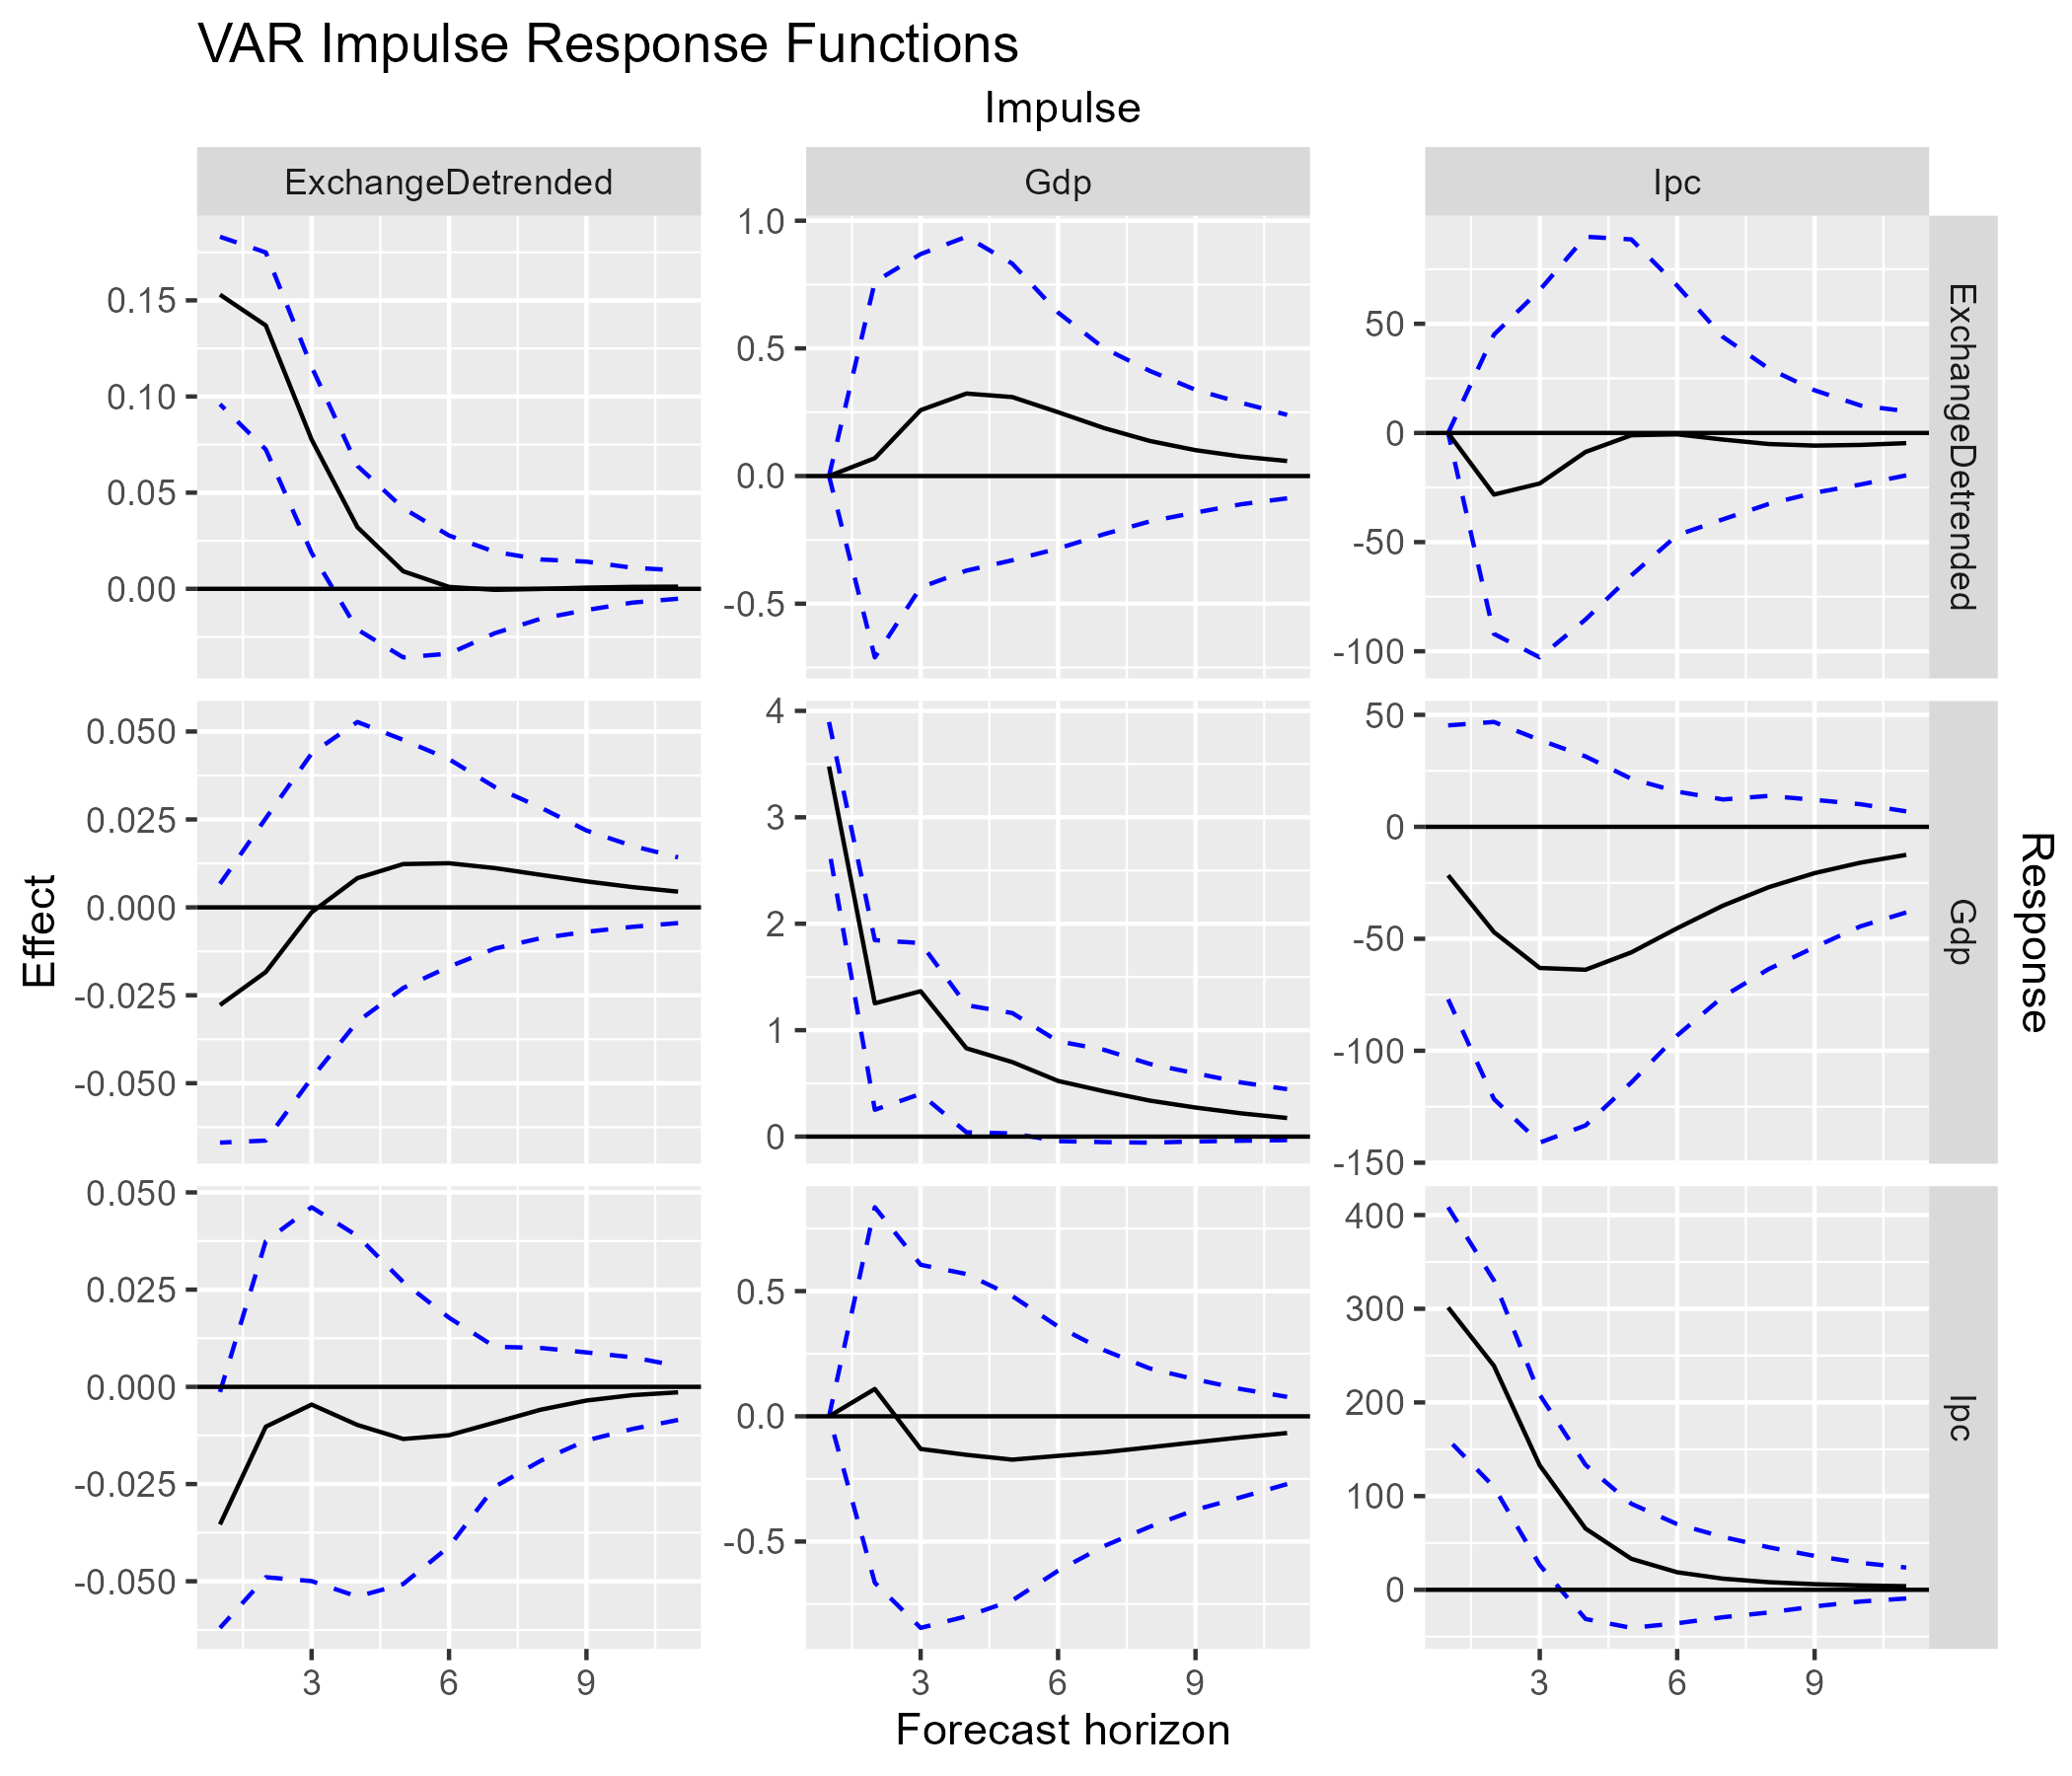
\includegraphics[width=0.8\textwidth]{figures/irfs.png}
\end{figure}

About credibility, the results show that ... .


\end{document}
